\documentclass[useAMS,usenatbib]{mn2e}
%\documentclass[a4paper,15pt]{article}
%\documentclass[a4paper,10pt]{article}
%\usepackage{aas_macros}
\usepackage{myaasmacros}
\usepackage{graphicx}
\usepackage{color}
\usepackage{amsmath}
%\usepackage{amssym}
%\usepackage{times}
%\usepackage{arial}
%\bibliographystyle{abbrv}
%\bibliographystyle{plain}
%\bibliographystyle{apalike}
%\bibliographystyle{mn2e}

% Some definitions of things I always use here:
\def\ltsima{$\; \buildrel < \over \sim \;$}
\def\simlt{\lower.5ex\hbox{\ltsima}}   
\def\gtsima{$\; \buildrel > \over \sim \;$}
\def\simgt{\lower.5ex\hbox{\gtsima}}
\def\siglos{\sigma_{\text{LOS}}}
\def\siglosi{\sigma_{\text{LOS},i}}

% Some definitions for the priors:
\def\gprior{{\tt gprior}}
\def\cprior{{\tt cprior}}
\def\bprior{{\tt bprior}}
\def\lbprior{{\tt lbprior}}

%Some definitions for rhodm etc:
\def\vztwo{\overline{v_z^2}}
\def\vztwoi{\overline{v_{z,i}^2}}
\def\rhodisc{\rho_\mathrm{disc}(z)}
\def\rhodmext{\rho_\mathrm{dm,ext}}
\def\rhodm{\rho_\mathrm{dm}}
\def\rhoeff{\rho_\mathrm{dm}^\mathrm{eff}}
\def\nuobs{\nu_\mathrm{obs}(z)}
\def\tot{\mathrm{tot}}
\def\kpc{\mathrm{kpc}}
\def\Msun{\mathrm{M}_{\odot}}

\newcommand\bcite[1]{(\citeauthor{#1} \citeyear{#1})}

\newcommand{\changefont}[3]{
\fontfamily{#1} \fontseries{#2} \fontshape{#3} \selectfont}

\newcommand{\TODO}[1]{\textsc{\textbf{\textcolor{red}{(TODO: #1)}}}}


\title[Dark Matter Distribution in Dwarf Spheroidals]
     {Dark Matter Distribution in Dwarf Spheroidals}
\author[P. Steger et al.]{P. Steger$^{1}$\thanks{E-mail: psteger@phys.ethz.ch},
 A. Boley$^{2}$,
 J. I. Read$^{1,3}$\\
 $^{1}$Department of Physics, ETH Z\"urich, CH-8093 Z\"urich,
 Switzerland\\
 $^{2}$Department of Astronomy; University of Florida, 211 Bryant
 Space Science Center, Gainesville, FL 32611, USA\\
 $^{3}$Department of Physics, University of Surrey, Guildford, GU2 7XH, UK
}
% \pagerange{\pageref{firstpage}--\pageref{lastpage}} \pubyear{2013}


\begin{document}

\maketitle

\label{firstpage}
\begin{abstract}
    I present results on dark matter distribution in dwarf galaxies
    found in simulations of representative patches down to redshift
    10. The influence of baryons on the dark matter profiles is
    investigated. Effects from mismatching halo centers are eliminated
    by applying different halo finder techniques and refinements.

    Substructures in the stellar components indicate that several star
    clusters formed independently before accreting on the center of a
    halo.

    The computed dark matter density profiles can be compared with
    observations, allowing us to check the underlying cosmological
    model. With known typical distribution, direct detection dark
    matter searches can be focused on the densest areas, allowing us
    to optimize for a higher annihilation detection rate.
\end{abstract}
%
\begin{keywords}
 cosmology: theory, large-scale structure of Universe --
 galaxies: dwarf spheroidals, evolution --
 methods: numerical
\end{keywords}
%
\section{Introduction}
\label{sec:intro}
What is Dark Matter? Where is it? How does it influence the buildup of
structures like the Milky Way?

\subsection{General Background}
An introduction to dynamics of bound systems is given in
e.g. \cite{Binney2008}, with emphasis on galaxies.


\TODO{some general concepts}

\subsubsection{Cosmological Models}
The cosmological model assumed in this work is based on the
$\Lambda$CDM model (\cite{Weinberg2008}, \cite{Peacock1999}), which
basically assumes that there is a varying amount of radiation,
baryonic matter, dark matter, and dark energy to fill up the energy
density of the Universe. The cosmology uses the 5-year WMAP values
\citep{Komatsu2009} for the cosmological parameters. \TODO{more info:
  really used 7-year WMAP values for generation of the ICs? find
  reference!}

\subsubsection{Structure Formation}
Structure is believed to form sequentially on small scales and to
contract to oblate structures (sheets), which meet in filaments, along
which the material accretes onto big clusters in the
intersections. This generates a structure called the Cosmic Web. A
more detailed review structure formation through the
history of the Universe is found in \cite{Padmanabhan1993}.

\subsection{Dark Matter}
The current measurements \citep{Komatsu2009} \TODO{WMAP7 update}
indicate that 83\% of the matter density is not interacting with
baryonic matter except through gravity and not emitting light,
therefore called dark matter.

\subsubsection{Evidence for Dark Matter}
Several objects in gravitationally bound systems were found to move
faster than the escape velocity determined by the potential of the
luminous parts. The investigation of high velocities of galaxies in
clusters e.g.\ led \cite{Zwicky1933} to assume the existence of a
hitherto unknown, not emitting material called {\sc dark
  matter}. Furthermore, galactic rotation curves should show
$v(r)\propto\sqrt{M(r)/r}$, with $v(r)\propto r^{-1/2}$ outside the
observed, luminous part; instead in most galaxies it rises to a
maximum value and stays approximately constant out to the edges of the
galaxy. This implies $M(r)\propto r$ or $\rho(r)\propto r^{-2}$.

\subsubsection{Models}
\paragraph{MOND}
Gravitational forces have been measured on small scales in
laboratories on Earth and tested in the solar system to
yield consistent results, if calculated via the framework of general
relativity. On larger scales, though, this has not been tested \TODO{citation}. {\sc
  Mond} (Modified Newtonian Dynamics, \cite{Milgrom1983}) assumes a
more general form of gravitational interaction

\begin{eqnarray}
  \vec{F}&=&\mu(a/a_0)m\vec{a},\\
  \mu(x\gg1)&\sim&1,\\
  \mu(x\ll1)&\sim&x
\end{eqnarray}

which reduces to the known gravitational $F(r)\propto r^{-2}$ on
small $r$. Instead of introducing a new particle type with exotic
features to account for the missing mass one could tune $\alpha$ such
that the interaction grows stronger with larger scales. The main
problems of this approach are i) that no simple physical process seems to
cause the expected behavior, and ii) that there remains the need for a yet
unseen form of matter in clusters of galaxies. The bullet cluster
\citep{Clowe2006} shows a mismatch of the loci of gravitating mass
and emission of a considerable fraction of gas in an ongoing merger
and thus indicates that dark matter is some new particle rather than
an effect from modified gravity.

\paragraph{Different velocity dispersions:}
Cold dark matter (CDM) is characterized by the fact that the proper
motion of the particles is much smaller than the expansion rate of the
Universe at freeze-out. CDM can collapse self-similarly on scales
ranging from super-clusters down to the smallest galaxies. It
decoupled from the temperature field in the early universe and started
to form small structures, which build structures on larger scales
subsequently.

Hot dark matter (HDM) consists of a particle type that is still freely
streaming, as are the neutrinos. Its high velocities hinder structure
formation below the mean free streaming path scale, which is the lower
bound for any cores seen.

Additional models of Warm Dark Matter range in between these two
extremes.

\paragraph{MACHOs and WIMPs:}
Massive astrophysical compact halo objects (MACHOs) such as brown
dwarfs, planets and other small objects too faint to be seen by
current telescopes contribute to the overall matter density in the
Universe.

Model calculations \TODO{citation} showed that they do not sum up to
the required amount of dark matter, supporting the existence of
another type of particles (Weakly interacting massive particles,
WIMPs).

This work implicitly assumes dark matter to be a particle given by the
(lightest) superposition of supersymmetric particles
\citep{Jungman1996}. \TODO{really?}

\subsubsection{Possibilities for Detection}
Experiments to detect dark matter directly are described e.g.\ in
\cite{Schnee2011}. One generally differs between direct and indirect
detection:

Direct detection searches for annihilation signals from high-energetic
particles generated during interactions with material in
detectors. The likelihood of interactions increase with the amount of
detector material, and is generally low due to the small interaction
crosssection predicted from cosmological constraints. Modern
photon-detectors are sensitive and need shielding from cosmic rays and
radioactive materials, which is generally accomplished by constructing
them well below the surface of the Earth. Other direct detection
experiments search for self-annihilation signals, i.e.\ particles
generated from different channels of interactions with dark matter
particles between themselves. These interactions are sensitive to the
density squared, which raises the need to know where a high
concentration of dark matter can be expected.

\TODO{Indirect detection experiments use}


To actually detect dark matter, one is interested in the expected
density distribution of dark matter in galaxies, as
\cite{Navarro1996} show.

Dynamics of stars in the solar neighborhood constrain the local dark
matter density. For big distances, on the other hand, weak and strong
lensing signals help to find the overall distribution of gravitating
matter, and subtracting the visible matter yields the
resulting dark matter profile.

\subsection{Dwarf Galaxies}
We adhere to the definition of dwarf galaxies as the smallest galaxies
in the Universe with dynamical masses of $10^6M_\odot-10^8M_\odot$
determined from visible components, while star masses range from
$\sim1000M_\odot$ to $10^7M_\odot$, and gas fractions of \TODO{gas
  fractions}.

An overview of the local group dwarf galaxies is given in
\cite{Mateo1998}. Star formation histories of the dwarfs is covered
e.g.\ in \cite{Skillman2005} and \cite{Dolphin2005}, kinematics in
\cite{Walker2009} and \cite{Simon2007}, and their orbits in
\cite{Lux2010}.

Elliptical galaxies with luminosities below $10^9L_\odot$ can be split
in two families, one of which has much lower surface brightness and
bigger radii than the other. This family is named dwarf
spheroidals. They are so faint that they are only detected in
the neighborhood of the Milky Way, with an estimated number count of
50-100 \citep{Belokurov2007}. They differ from other gravitationally
bound systems in that they consist mostly of dark matter.

\subsubsection{Observations}
In galaxies with a mass as low as stated before, the luminosity is
expected to be very low as well. This induces that only nearby dwarf
galaxies can be observed with current observational instruments.

Observations showed some 10 classical dwarfs in the Milky Way halo
\TODO{citation}. Recently, wide area surveys discovered more and more
dwarfs, \citep{Belokurov2007}, \citep{Belokurov2009},
\citep{Belokurov2010}, totalling 25 in a 20\% coverage of the sky
\citep{Koposov2008}. Following predictions of $\Lambda$CDM, there
should be thousands of them, though \cite{Diemand2007}. This
discrepancy is generally known as the ``missing satellites problem'',
\citep{Moore1999}, \citep{Klypin1999}.

Moreover, observations give hints to the existence of a core in the
central parts of rotationally supported dwarf galaxies. This is in
contrast to theory predicting cuspy profiles for dark matter only
profiles, \citep{Moore1994}, \citep{Flores1994}, \citep{Moore1999a}.  

It is not possible to disentangle the effects of the proposed mass
profile from the anisotropic velocity distribution reliably.

The systems under study in e.g. \cite{deBlok2001} are gas-rich low
surface brightness galaxies, with higher mass and more gas than our
simulated dwarfs.

Looking at simulated small galaxies that are not necessarily
rotationally supported, additional constraints as to which properties
distinguish cores and cusps can be found. Baryons do play an
non-neglectible role in dwarf dynamics, with proposed processes
generating cores from cusps via i) non-adiabatic contraction ii)
recurring baryonic in-/outflow \citep{Read2005}, which could render the
cusp-core problem pointless. This is in fact seen in simulations
\citep{Mashchenko2008}, \citep{Governato2009}, which shows that the
early assumption that baryon physics has only small influence were
inaccurate \citep{Navarro1996}, \citep{Gnedin2002}.

\cite{Teyssier+2013} find that the scale of the outflows correlate
with the size of the cored region.

\subsection{Globular Clusters}
Massive star clusters in the halo of the Milky Way - of which some 150
are detected by now. \citep{Zinn1985} and \citep{DeAngeli2005} show a
mass in stars that is comparable to the dwarf spheroidals, typically
$10^5$ to $10^6M_\odot$. The resemblance is going further as they have
a similar age; they are mostly old, as old as the Universe itself. The
big difference lies in the fact that they show little to no evidence
for dark matter in them, whereas dynamics of dwarf spheroidals implies
a mass fraction of $90\%$ in dark matter. \TODO{place, location}

Why should stars form in environments with such a wide spread in
density? Is there a connection between dwarf spheroidals and globular
star clusters? Given there is one, how can it be determined
qualitatively and quantitatively? It has been proposed \TODO{citation}
that one is the evolved form of the other; or \TODO{citation} that they
form in different environments.

By extracting basic properties that differ in between globular star
clusters and dwarf spheroidals, one can try to answer that
question. The temporal evolution of the defined substructures gives
hints as to whether they represent different phases in an evolutionary
path.

The density of globular clusters is such that in a typical patch of
the LCDM Universe of size $1\rm Mpc$ at $z=10$ contains a few of them
\citep{Boley2009}. \TODO{really? not meant dwarf galaxies?}

\subsection{Simulations}
The general paradigm behind simulations is as follows:

Simulations try to recover observations of todays structures and check
theoretical models. This is done via setup of initial conditions with
power spectrum similar to the the cosmic microwave background. In a
first approximation, Gaussianity is assumed. For higher order terms,
non-gaussianity is included via the correction term $f_{\rm NL}$.
\TODO{state of the art, reason why not included}
  
These initial conditions are power spectra for the modes of
displacement in density and velocity, modeled on a grid of $N^3$
particles -- and possibly further refinements -- in a box. The box is
assumed to repeat itself in each cartesian coordinate, effectively
forming a hypertorus.

The simulation is then started and evolves the current state by
calculating

\begin{itemize}
\item gravitational forces between particles
\item hydrodynamical quantities, either for hydro particles or on a mesh
\item the resulting changes for the next step
\end{itemize}

A review of how structure formation can be modeled by numerical means
is found in \cite{Bagla2005}.

Collisional codes follow each of the particles directly, while
collisionless simulations follow a smaller number of particles that
are actually observed in the system. Collisional codes are used to
follow systems in which close encounters play a significant role and
need to be resolved, i.e.\ when the relaxation time is of order of the
simulation timestep. In collisionless simulations one models a
continuum distribution by sampling only a small number of
particles. Dark matter as a pressureless fluid is often treated with
this paradigma.

$N$-body simulations use a discrete sample of points in phase space
to follow the evolution of the whole system. The track of a particle
is determined by the gravitational force on it generated by the
gravitational potential of all other particles. Any code that
calculates this force and then follows the particle path and thereby
integrates Poisson's equation is called a Poisson solver.

Particle-Particle-Particle-Mesh codes (PPPM) use direct summation of forces
between all (star/dark matter) particles.

* \TODO{PM}

* Smoothed particle hydrodynamics ({\sc Sph}) approaches the fluids by
particles representing volume elements, and calculates the
hydrodynamical forces from a discrete form of the Euler
equations. Gadget is a prominent example of such a code.

Grid codes in contrast follow the gas dynamics in small patches and
updates the hydro variables in the neighboring cells according to the
flux through boundaries and volume changes. Meshes can take a
diversity of geometries, depending on the physical system under
consideration.

Adaptive mesh refinement (AMR) describes an advanced technology to
follow the liquid more accurately: The mesh is refined in the vicinity
of high overdensities or at discontinuities in the density, allowing
for correct capture of accretion, shock waves, and other small
features.

\subsection{Overview this work}

This work is organized as follos: After this introduction with an
overview over the widespread field of dark matter research and methods
of numerics in cosmology, we start by describing the simulations
performed in section \ref{sec:data}, followed by a short explanation
on the methods in section \ref{sec:meth}. We then focus on results:
section \ref{sec:res} first concentrates on halo finding performance
and general properties of the halos in a high resolution,
hydrodynamical simulation, both for dark matter/stars and gas. This is
compared with the properties found in a dark matter only simulation of
the same intitial conditions, allowing to draw conclusions on the
influence of baryons.

%
%% SIMULATIONS
%
\section{Methods}
\label{sec:meth}

\subsection{The Simulations}

\begin{figure*}
  \begin{center}
    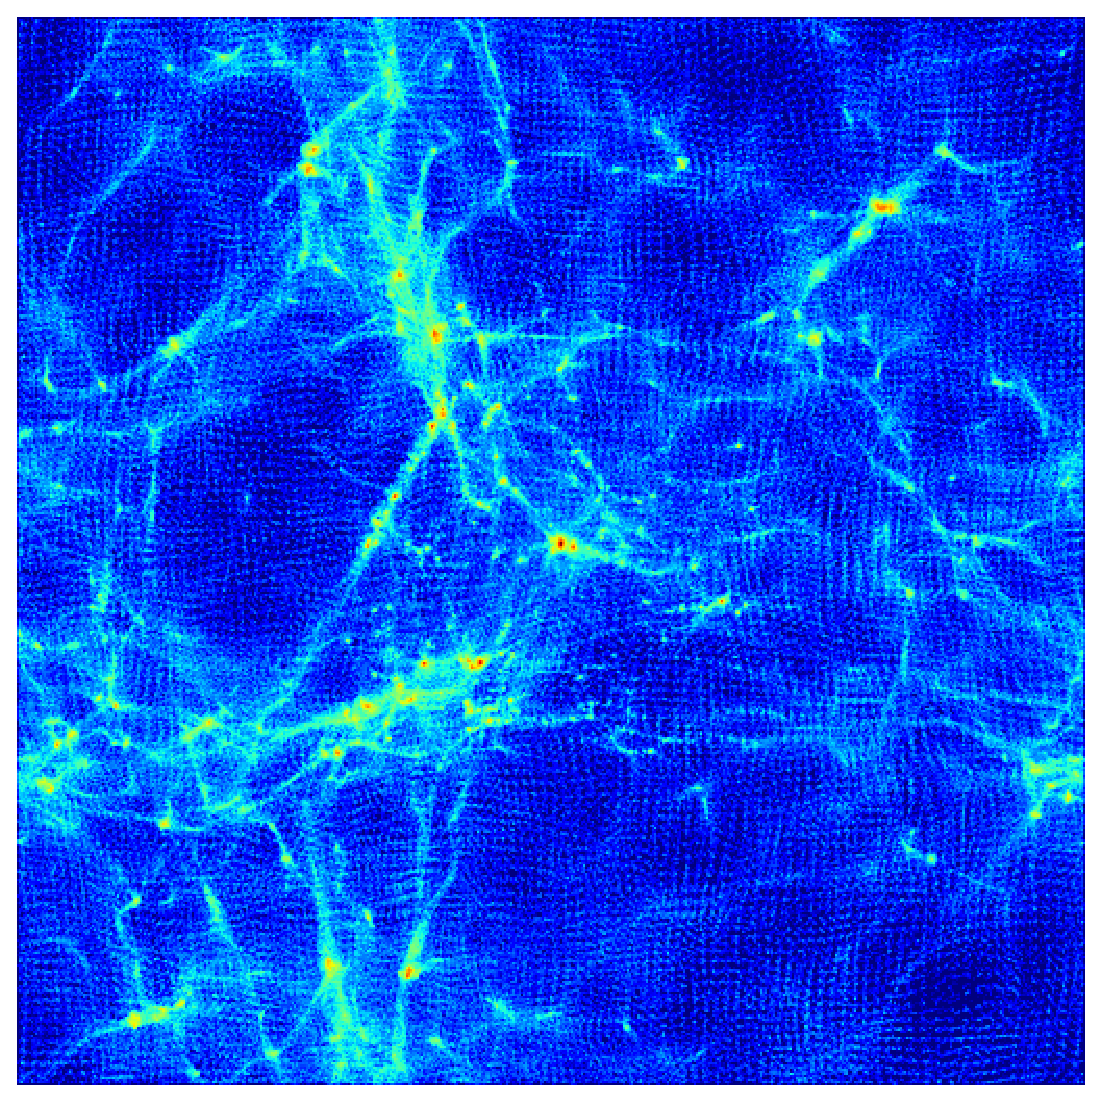
\includegraphics[width=0.45\textwidth]{fig/vis_dm.eps}
    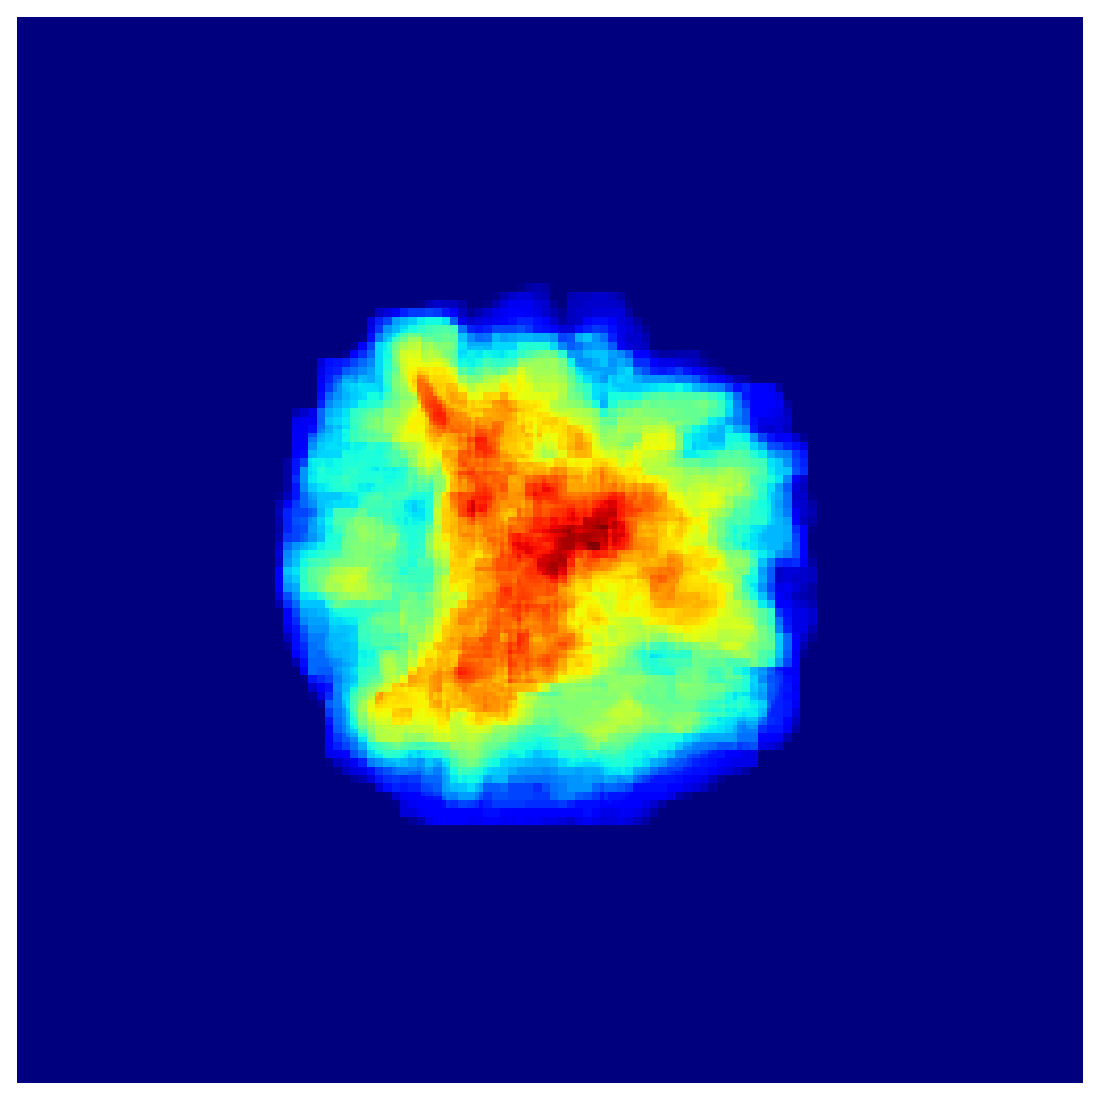
\includegraphics[width=0.45\textwidth]{fig/vis_gas.eps}
  \end{center}
  \caption{\label{fig:vis} Visualization of one of the simulation box
    in the high resolution hydro run, with dark matter density in the
    left panel, and gas density encoded in a grid in the right
    box. The visible box size spans a range of $1\,{\rm Mpc}/h$.}
\end{figure*}

Six simulations were run for this project. The main simulation was run
with high resolution in a refined region, and including nonequilibrium
chemistry to follow evolve reliable cooling rates down to temperatures
below $10^4$K. For comparative reasons the same resolution was used
for a dark matter only simulation, and convergence was investigated by
comparing that one to a lower dark matter only simulation. All
simulations used the same cosmology, as follows.

\subsubsection{Cosmological Parameters}
The high resolution hydrodynamical simulation was run with WMAP-5 \TODO{check valus in ICs}
concordance cosmology parameters, i.e. $\Omega_\Lambda=0.742$,
$\Omega_M=0.258$, $\Omega_b=0.045$, $h=0.719$, $\sigma_8=1.0$.

\subsubsection{Initial Conditions}
Initial conditions were generated with {\sc Cosmics}
\citep{Bertschinger1995}, for a box of $1{\rm Mpc}/h$ boxlength, at
$z=1000$, with a low resolution boundary layer of $256^3$ equivalent
particles and an inner high resolution region of $256^3$ particles,
which again was refined by a factor 2 to match $245^3$ particles in
the second nested layer. The dark matter only, high resolution run was
performed with $256^3$ particles on the whole box. The mass resolution
is thus set to \TODO{check} $120\Msun$. This corresponds to the
average stellar mass to produce a supernova. By this procedure, we
ensure that every supernova in our simulation corresponds to an actual
star exploding.

\subsubsection{Temporal coverage}
The simulation is run from $z=1000$ down to $z=10$, with outputs on
$100$ equally spaced intervals, allowing to track specified structures
back in time.

It has been shown in \cite{Boley2009} that in a typical volume of
$1{\rm Mpc}/h$ at $z\sim10$ there should be a few dwarf spheroidal
galaxies present. Thus the progenitors of todays dwarfs were generated
before reionization. Its influence on the baryonic component will be
considered in future work, e.g. via a windtunnel emulating the effects
of ram-pressure stripping and shock front buildup during
infall. \TODO{so much/more detail?}

\subsubsection{Simulation physics}
The same physics as in \cite{Boley2009} was used for the high
resolution hydrodynamical simulation. This includes ram pressure, star
formation, SN feedback, AGN. {\sc Ramses} has beed used in a augmented
version to follow nonequilibrium physics as well, namely the gas of
$e$, {\sc Hi}, {\sc Hii}, {\sc Hei}, {\sc Heii}, {\sc Heiii}, $\textrm{H}^-$,
H$_2$, and ${\textrm H}_2^+$ \citep{Abel1997}. We do not include $\textrm{HD}$.

\TODO{network with reaction rate references}

\subsection{Higher Resolution}
We use significantly higher resolution than was previously performed
\citep{Boley2009}, with non-equilibrium physics included.

The force resolution (Plummer's equivalent length) in the highest
resolution mesh is \TODO{update} $4{\rm pc}/h$ at $z=10$, which sets a
restriction on the determination of densities in the inner regions for
the smallest halos. It is indicated as a vertical line in the graphs
of radial profiles.

\begin{table*}
  \begin{center} \begin{tabular}{lcccccr} \hline 
      ID & description & box size $[{\rm Mpc}/h]$ & $z_{\rm start}$ & $z_{\rm end}$ & $n_{\rm DM}$ & $\varepsilon$ $[{\rm pc}/h]$\\
      \hline
      hydro   & full hydro physics high resolution & 1 & 100 & 10 & \TODO{fill} & 4\\
      dm low  & dark matter only low resolution    & 1 & 100 & 10 & \TODO{fill} & \TODO{fill}\\
      dm high & dark matter only high resolution   & 1 & 100 & 10 & \TODO{fill} & \TODO{fill}\\
      \hline
    \end{tabular} \end{center}
  \caption{\label{tab:simprop}Properties of the simulations under study. $\varepsilon$ gives the equivalent Plummer's width.}
\end{table*}


\subsection{Definitions}
\subsubsection{Bound Structures}
The virial radius $r_{vir}$ is determined to be the distance from the densest point of a halo at which the mean enclosed density $\rho(r)$ is according \cite{Bryan1998}
%
\begin{eqnarray}
  \rho(r)&>&\Delta(z)\rho_{crit,0}\\
  \Delta(z)&=&18\pi^2+82x-39x^2\\
  x&=&\Omega(z)-1\\
  \Omega(z)&=&\Omega_0(1+z^3)/E(z)\\
  E(z)&=&\sqrt{\Omega_0(1+z^3)+\Omega_R(1+z)^2+\Omega_\Lambda}
\end{eqnarray}

\subsubsection{Radial Profile}
The radial density profile $\rho(r)$ is determined from
logarithmically spaced shells around the detected centers.

\begin{equation}
  r_i=\TODO{fill}
\end{equation}

\subsubsection{Halo Finding}
The simulation outcome by itself shows only properties of individual
dark matter particles, and additionally a mesh for the hydrodynamical
constituents. One is interested in bound substructures, which have to
be found first by a halo finding technique.

\paragraph{FOF:}
The friend-of-friends algorithm as e.g.\ described in \cite{Press1982}
starts with a particle and searches for its nearest neighbor, out to a
predefined radius. After doing this iteratively, all particles
connected by such a chain are considered to lie within the same
halo. This procedure works well for isolated halos only; two nearby
halos connected by a filament could be detected as one structure
only. Recent findings \citep{More2011} \TODO{include in bibliography}
show that the overdensity inside the virial radius is typically of
order $80$ instead of the generally expected $180$. \TODO{other
  flavors, state of the art}

\paragraph{HOP:}
{\sc Hop} from the {\sc Ramses} toolkit starts off by computing the
density around each particle with an adaptive kernel, then hops to the
neighbor particle at highest density, and assigning all particles
ending at the same point to the same structure. Breaking up due to
local density maxima is overcome by merging two groups if the density
of the boundary layer between them lies above a given threshold.

\paragraph{Watershed:}
The watershed algorithm \cite{Platen2007} starts from the density
maxima as leaves of the halo/subhalo tree. Stepping further out, all
material in the same potential pot is assigned to the respective
maxima. As soon as a neighbor maximum is encountered, both halos form
an additional leave in the tree.

\paragraph{SOD:}
The spherical overdensity algorithm as introduced by \cite{Lacey1994}
grows a sphere around particles at density minima and stops if the
mean density falls below a threshold. This procedure is repeated with
the remaining particles until no structure with a minimum number of
particles is found anymore. It does not handle correctly the cases of
mergers, yielding a halo position in the middle of both merging halos.

Here the {\sc AHFstep} algorithm of the simulation code {\sc Amiga}
\TODO{citation} is used. It showed superior capabilities with mock
halos and subhalos \TODO{citation}. 

%The {\sc Ramses} simulation snapshots are first converted to Gadget
%format, allowing a simple read-in for {\sc AHFstep}.

The prospective halo centers can be defined in several ways: by the
position of the center of mass, the center of the potential or the
density maximum. Visually best agreement with dark matter density
projection was found for the position of maximal density.

An additional iterative procedure excludes all particles which are
kinematically unbound: if the kinetic and internal energy (for hydro
particles) exceed the potential energy, the particle is removed, the
potential recalculated and further unbound particles excluded.

Additional displacements with respect to the densest point were
corrected with an additional shrinking sphere algorithm: It starts
from the center of mass of all particles in a sphere of radius $r_{\rm
  vir}$, then rescales the radius to $r_{i+1}=f\cdot r_i$, $f\leq
1$, and considers only particles inside the smaller sphere to find the
center of mass in the next step, until the positions converge to
$(\Delta x_{i\to i+1}-\Delta x_{i-1\to i})/\Delta x_{i\to
  i-1}<\varepsilon$. Similar restrictions on the convergence of COM
velocity were not considered. The two parameters $f$ and $\rho$ are
not restricted by a physical argument and thus have been chosen such
that for the majority of massive halos convergence was reached in
$<100$ steps, with displacements $<0.1r_{\rm vir}$. \TODO{redo}

\subsection{Halo Selection}
We are interested in the inner density profile of dwarf spheroidals,
therefore, only halos with virial mass above $10^7M_\odot/h$ and no
host halo are considered further. Their main properties are listed in
table \ref{tab:haloprop}.

\begin{table*}
  \begin{center} \begin{tabular}{lccccccccr} \hline Simulation &
      ID & $M_{\rm vir} / h^{-1}{\rm M}_\odot $ & $R_{\rm vir} /
      h^{-1}{\rm pc}$ &x&y&z& $f_{DM}$ & $f_{gas}$ & $f_{stars}$ \\ 
      \hline
      hydro & 1 & $4.070\cdot10^7$ & $8.52\cdot10^3$&0.5095&0.5064&0.4941&&& \\
      hydro & 2 & $1.522\cdot10^7$ & $6.14\cdot10^3$&0.5214&0.5040&0.4801&&& \\
      hydro & 3 & $1.410\cdot10^7$ & $5.98\cdot10^3$&0.3987&0.6329&0.6409&&& \\
      hydro & 4 & $1.336\cdot10^7$ & $5.88\cdot10^3$&0.3886&0.6167&0.6376&&& \\
      hydro & 5 & $1.108\cdot10^7$ & $5.52\cdot10^3$&0.4338&0.3954&0.4415&&& \\
      \hline
      dm&1&$5.579\cdot10^7$&$9.46\cdot10^3$&0.3629&0.3630&0.3579&1.0&0.0&0.0\\
      dm&2&$4.205\cdot10^7$&$8.61\cdot10^3$&0.2648&0.0773&0.4323&1.0&0.0&0.0\\
      dm&3&$3.036\cdot10^7$&$7.73\cdot10^3$&0.2844&0.4540&0.4588&1.0&0.0&0.0\\
      dm&4&$2.822\cdot10^7$&$7.54\cdot10^3$&0.1983&0.6295&0.3276&1.0&0.0&0.0\\
      dm&5&$1.999\cdot10^7$&$6.72\cdot10^3$&0.2574&0.5456&0.5674&1.0&0.0&0.0\\
      \hline
    \end{tabular} \end{center}
  \caption{\label{tab:haloprop}Properties of the selected halos. $M_{\rm vir}$ and $R_{\rm vir}$ are the virial mass and radius of the halos, $f_i$ gives the fraction of mass in component $i$.}
\end{table*}

\subsection{Relaxation Radius}
The relaxation radius was determined according to definitions and
methods described in \cite{Read2009}. $N$ is the total particle number
enclosed in a sphere of radius $r$ around the center with a mass of
$M(<r)$, $b_{\rm max}$ and $b_{\rm min}$ are maximal and minimal
impact parameter, which are set to virial radius and gravitational
force softening length in a first step.

\begin{eqnarray}
  t_{\rm relax}&=&n_{\rm cross}t_{\rm cross}\sim\frac{N}{16\pi\ln\Lambda}t_{\rm orb}\\
  t_{\rm orb}&=&2\pi b_{\rm max}\sqrt{\frac{b_{\rm max}}{GM(<r)}}\\
  \ln\Lambda&=&\ln\frac{b_{\rm max}}{b_{\rm min}}\\
  t_{\rm relax}(r)&=&\frac{N b_{\rm max}^{3/2}}{8\sqrt{GM(<r)}\ln(b_{\rm max}/b_{\rm min})}\\
  t_{\rm sim}&=&t_{\rm relax}(r_{\rm relax})
\end{eqnarray}

The last equation is solved for $r_{\rm relax}$ by a basic root
finding algorithm. All quantities determined from particles inside
$r_{\rm relax}$ are expected to be widely independent of the
properties of the surrounding halo, as any memory was erased in
numerous encounters. The relaxation radius can be defined in several
ways for simulated systems, with better matches when $b_{\rm max}=r$,
allowing the Coulomb logarithm $\ln\Lambda$ to change slowly with
radius.

\section{Results}
\label{sec:res}

\subsection{DM density profile}
Dark matter density profiles are shown in
fig. \ref{fig:hydro_dmonly_prof} for the most massive halo in each
simulation at $z=10$. The vertical blue line indicates the force
softening length on the most refined grid in the hydrodynamical
run. All values at smaller radii are not to be trusted.

\begin{figure*}
  \begin{center}
    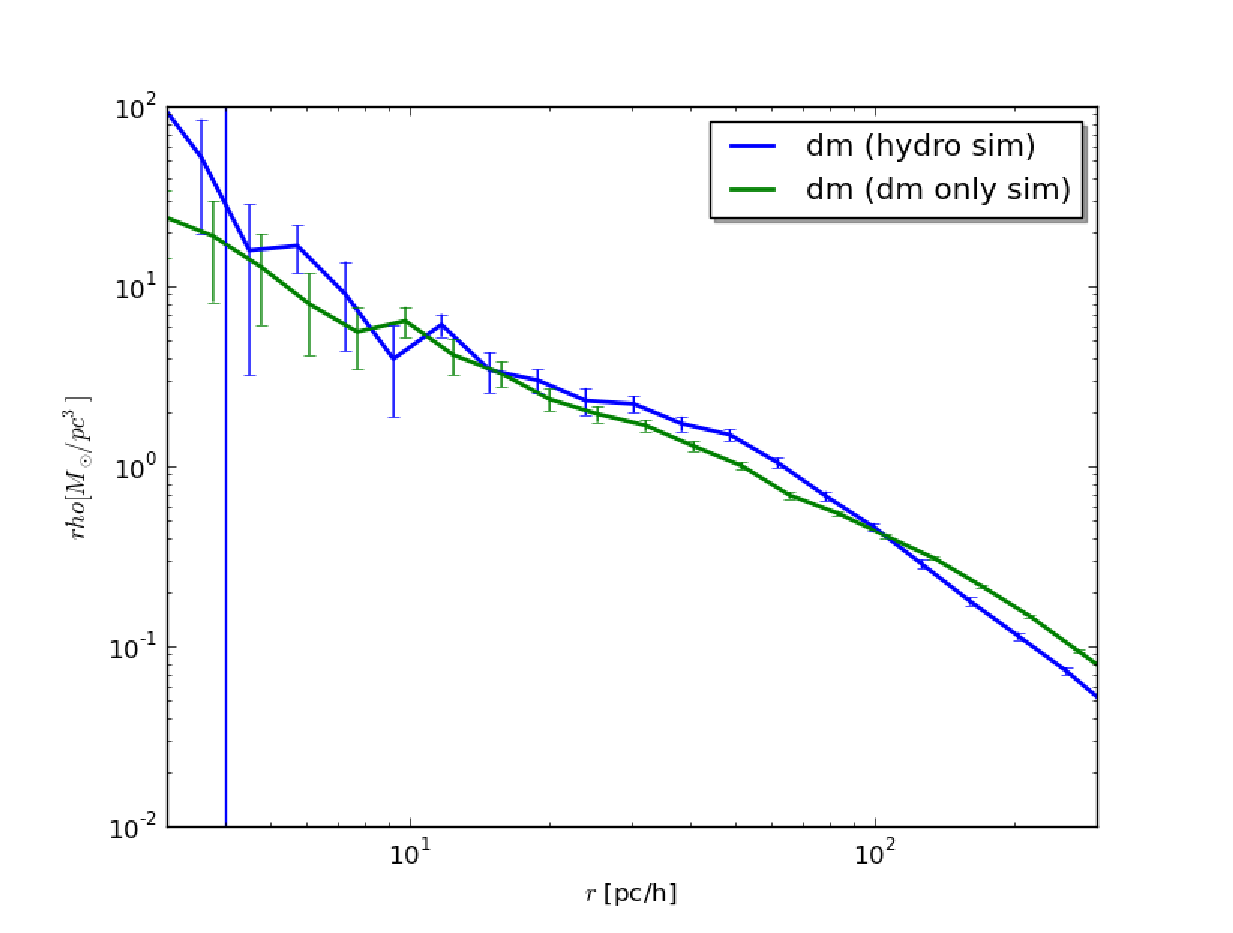
\includegraphics[width=0.4\textwidth]{fig/hydro_dmonly_prof.eps}
    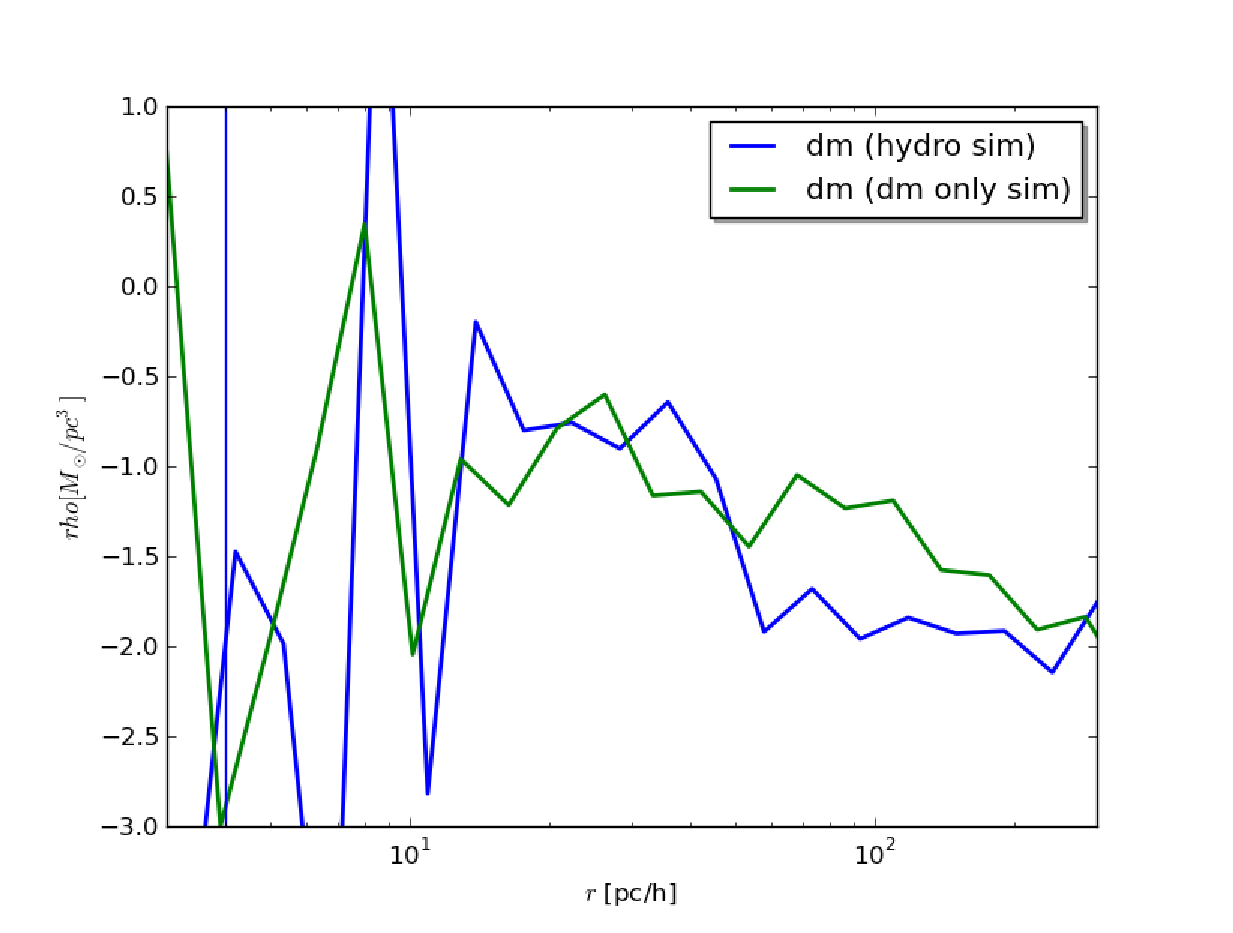
\includegraphics[width=0.4\textwidth]{fig/dlnrhodm.eps}
  \end{center}
  \caption{\label{fig:dm_prof}Dark matter density profiles for the
    most massive halo in both runs.}
\end{figure*}


Fig. \ref{fig:prof_dmonly} shows the profiles for the halos {\sc dm 1-5}.
\begin{figure*}
  \begin{center}
    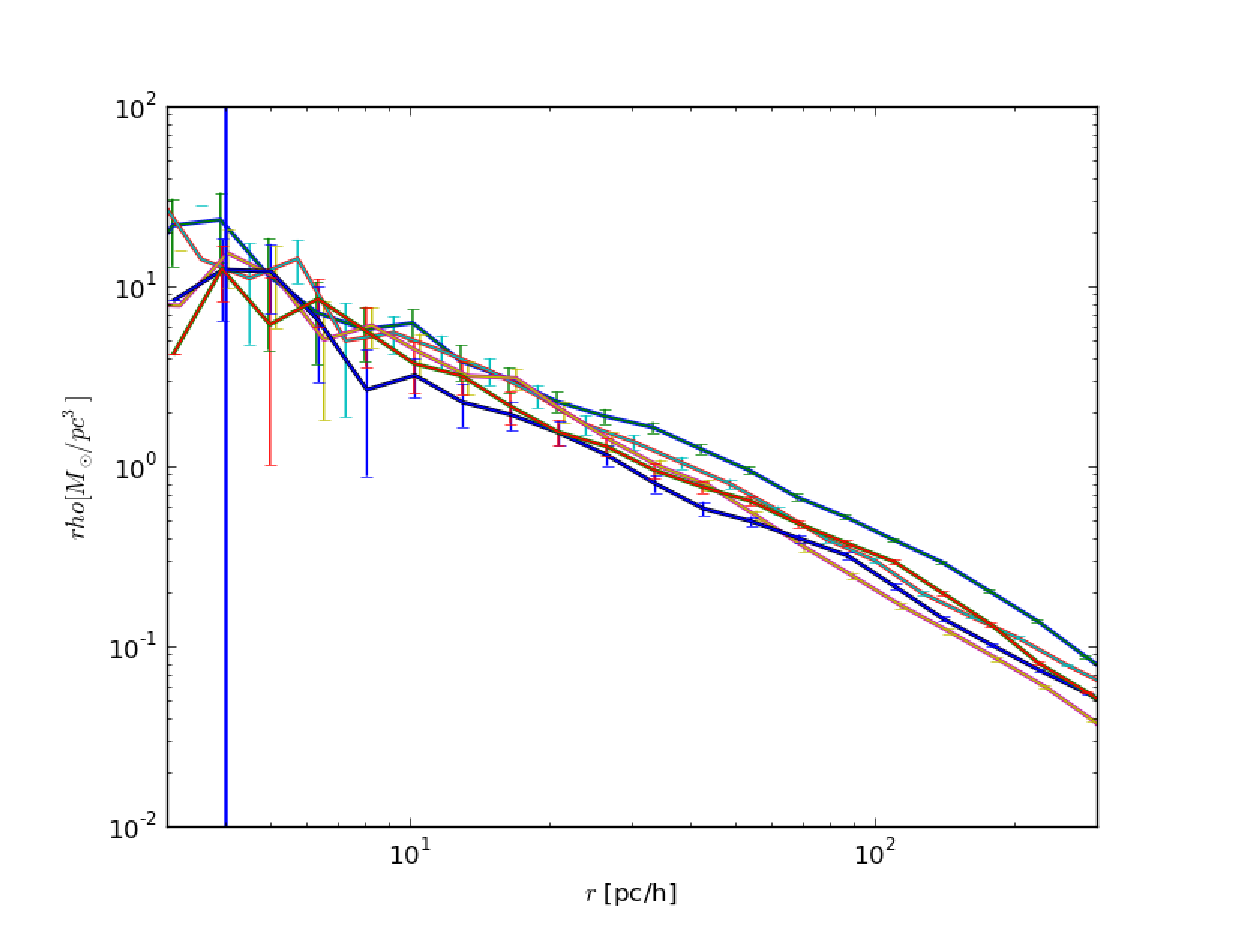
\includegraphics[width=0.4\textwidth]{fig/prof_dmonly.eps}
    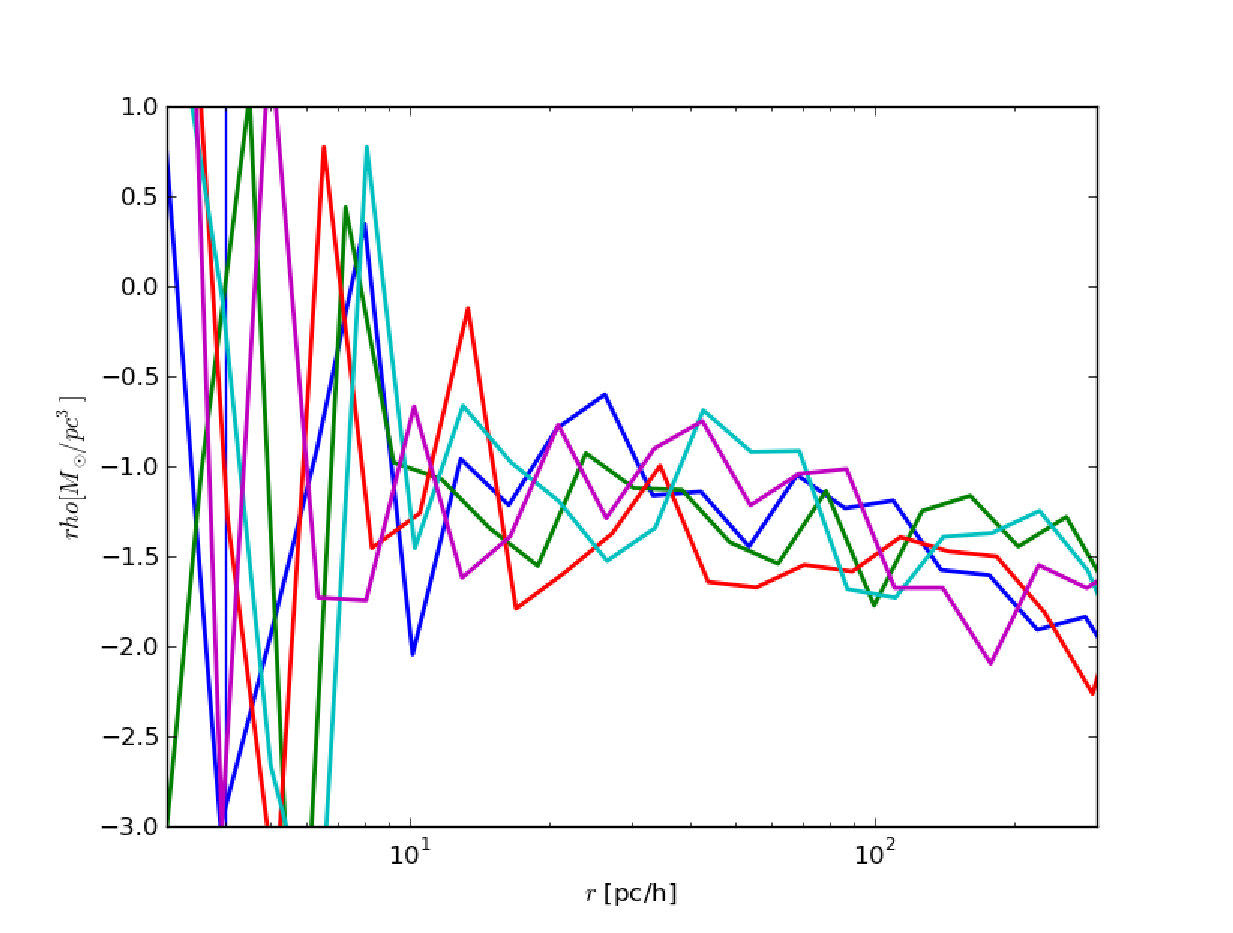
\includegraphics[width=0.4\textwidth]{fig/dlnrhodm_all.eps}
  \end{center}
  \caption{\label{fig:prof_dmonly}Dark matter density profile of the five most massive halos}
\end{figure*}

Fig. \ref{fig:star_prof} shows both dark matter and star density profiles for {\sc hydro 1} and {\sc hydro 5}. \TODO{Adiabatic contraction}
\begin{figure*}
  \begin{center}
    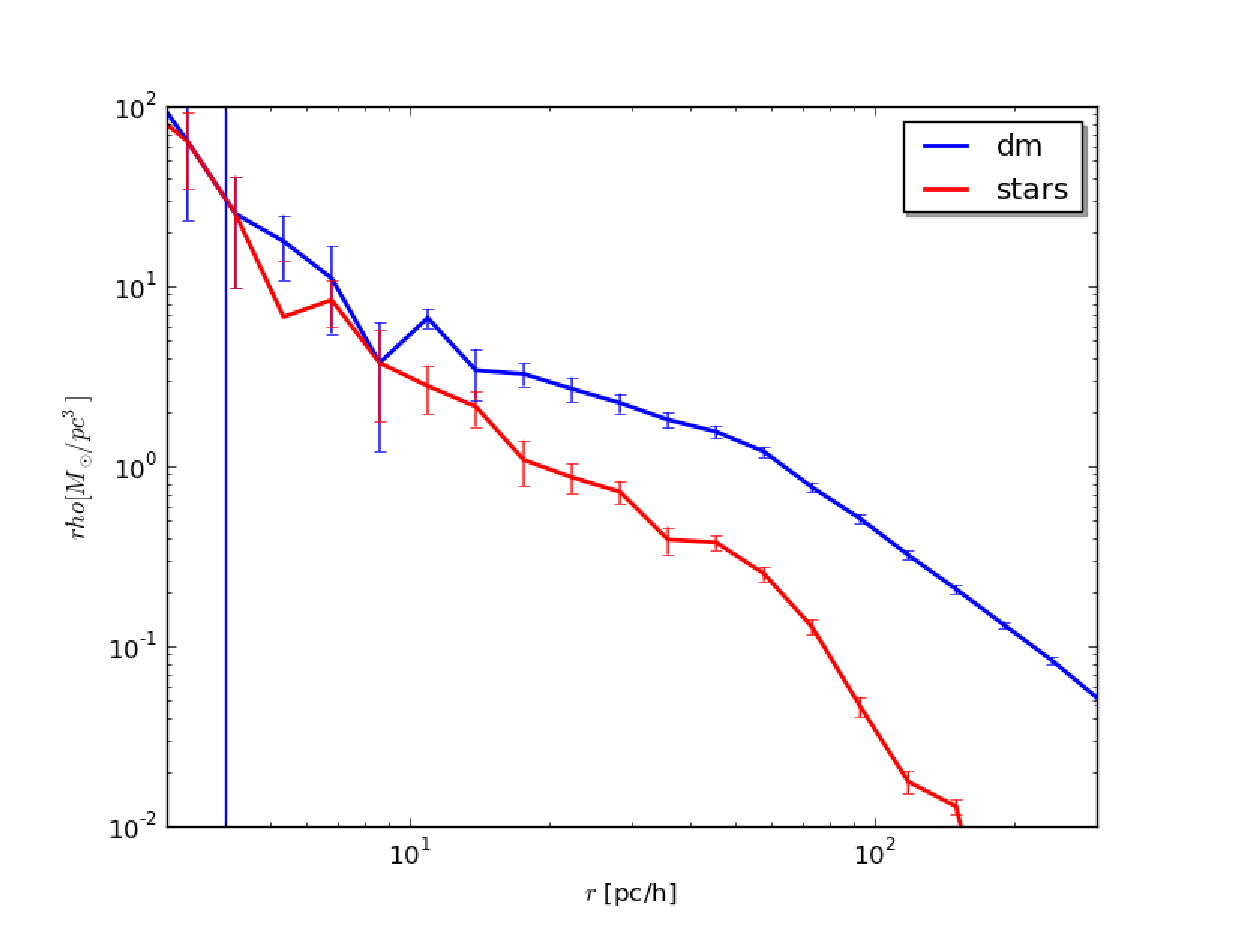
\includegraphics[width=0.4\textwidth]{fig/map_dm_stars_1.eps}
    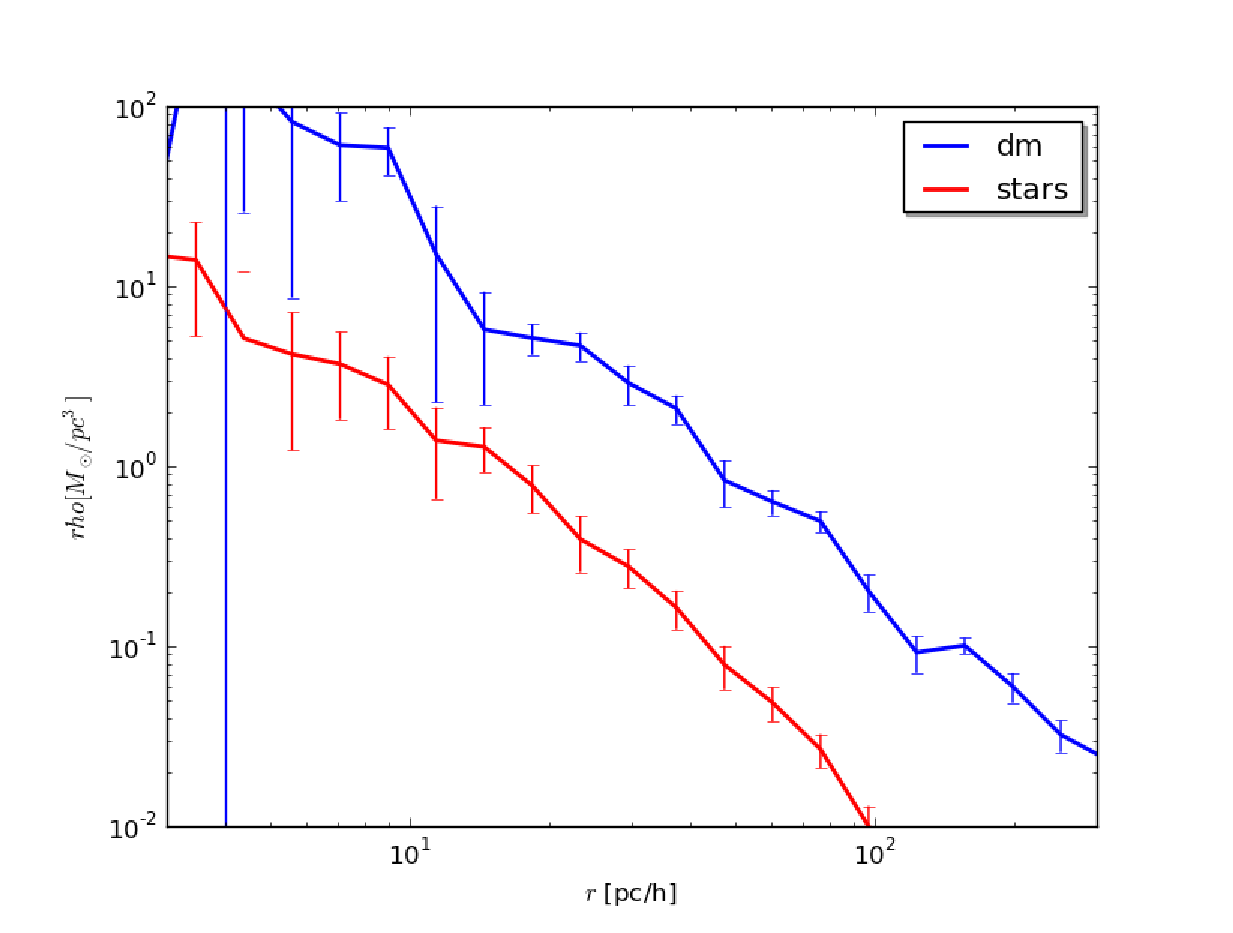
\includegraphics[width=0.4\textwidth]{fig/map_dm_stars_5.eps}
  \end{center}
  \caption{\label{fig:star_prof}Density profile of dark matter and star particles in ({\sc hydro 1}) and ({\sc hydro 5})}
\end{figure*}

%\begin{figure}
%  \begin{center}
%    
\includegraphics[width=0.1\textwidth]{fig/a.eps}%hist_mstarbymdm.png}
%  \end{center}
%  \caption{\label{fig:hist_mstarbymdm}Fraction of stellar mass to
%  dark matter mass in all halos with $M<\TODO{Mmax}$}
%\end{figure}

\subsection{Halo finding}
It is important to center the halos correctly on the most dense point,
as a little offset implicates an overdensity at the radius of offset,
thus turning a cusp into a broader core.
Fig. \ref{fig:vis_proj_dm_sod_ahf} shows positions and virial radii
detected with two of the above mentioned methods, spherical
overdensity ({\sc Sod}, pink circles) and {\sc Ahf} (red crosses).

\begin{figure}
  \begin{center}
    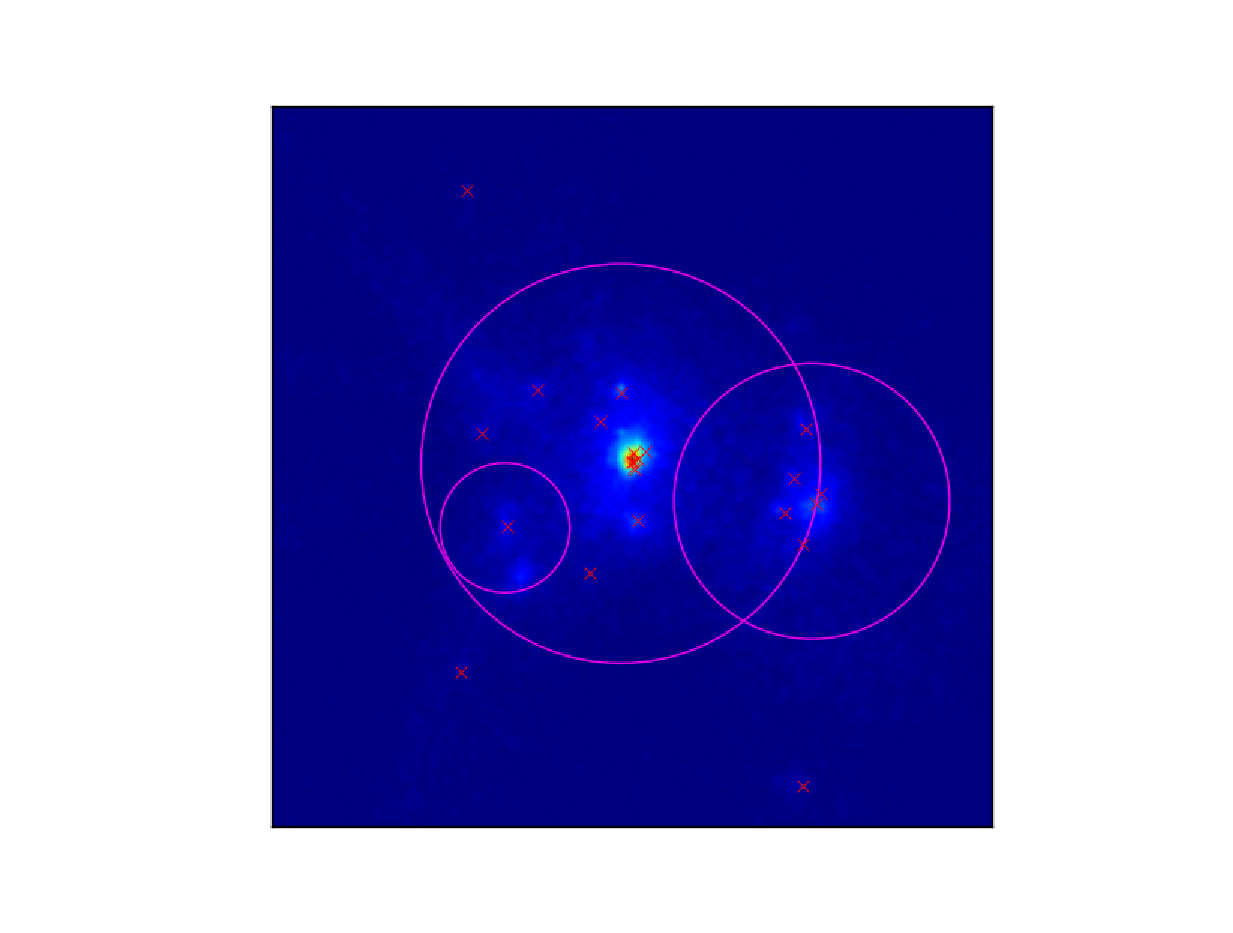
\includegraphics[width=0.5\textwidth]{fig/sod_ahf.eps}
  \end{center}
  \caption{\label{fig:vis_proj_dm_sod_ahf}Positions of the halos
    detected by SOD (blue circle) and {\sc Ahf} (red crosses) on top
    of dark matter density. The radii of the circles corresponds to
    the value of $r_{vir}$ as detected by {\sc Sod}.}
\end{figure}

Fig. \ref{fig:ov_1} and \ref{fig:ov_5} give an overview of {\sc hydro
  1} and {\sc hydro 5} as the most massive and least massive halo
considered. Projections along the three axes $x,y,z$ of dark matter
density, star density and {\sc Amr} grid (proportional to gas density)
are shown.
\begin{figure*}
  \begin{center}
    \includegraphics[width=1.0\textwidth]{fig/ov_1.eps}
  \end{center}
  \caption{\label{fig:ov_1}Projections of dark matter density (top
    row), star density (middle row) and {\sc Amr} grid (bottom row)
    along all three axes for halo {\sc hydro 1}.}
\end{figure*}

\begin{figure*}
  \begin{center}
    \includegraphics[width=1.0\textwidth]{fig/ov_5.eps}
  \end{center}
  \caption{\label{fig:ov_4}Projections of dark matter density (top
    row), star density (middle row) and {\sc Amr} grid (bottom row)
    along all three axes for halo {\sc hydro 5}.}
\end{figure*}

Additional centering with the shrinking sphere algorithm for values of
$f=0.1$ and $\varepsilon=0.01$ resulted in displacements as shown in
fig. \ref{fig:hist_shrsph}. This method relies on a sensible choice of
both of these values, which need to be set for each halo
separately. There is no considerable change for the massive halos, and
only the centers of small subhalos get affected.

\begin{figure}
  \begin{center}
    
\includegraphics[width=\textwidth]{fig/a.eps}%hist_shrsph.png}
  \end{center}
  \caption{\label{fig:hist_shrsph}Distribution of additional position
    correction by shrinking sphere algorithm. \TODO{regenerate}}
\end{figure}

\subsection{Stars}

Fig. \ref{fig:star_proj_1} shows a projection of all stars in {\sc
  hydro 1}, plotted on the overall density distribution. The size of
the stars is proportional to their metallicity. Assuming that groups
of stars forming at roughly the same time in the same region should
show approximately the same metallicity, one draws the conclusion that
they first formed outside the halo before being accreted.

\begin{figure}
  \begin{center}
    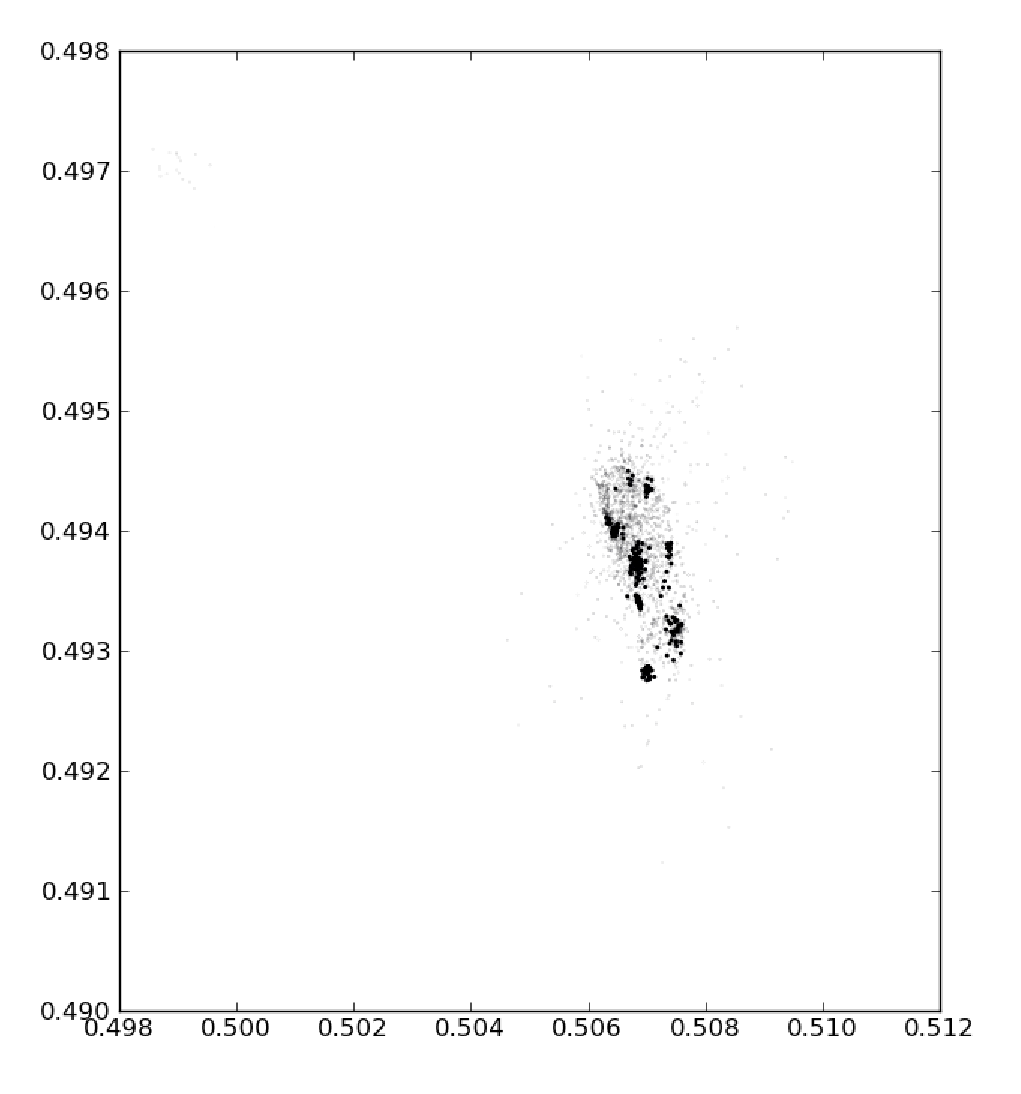
\includegraphics[width=\textwidth]{fig/star_proj_1.eps}
  \end{center}
  \caption{\label{fig:star_proj_1}Projection of stars in {\sc hydro
      1}, centered on the overall center of mass. The size of the
    stars is scaled according to metallicity. There are different
    groups of stars with each approximately the same metallicity.}
\end{figure}


\section{Summary and Discussion}
\label{sec:sum}

\subsection{Impacts on Formation History}

\subsection{Local DM Density}
The local dark matter density \cite{Garbari2010} is a superposition of
dark matter from the disc and the halo of the Milky Way. Simulations
of dwarf galaxies as studied above falling through the disc could help
to constrain the evolution of the vertical density profile.

\section*{Acknowledgements}
\label{sec:ack}

I warmly thank J. Read for many helpful discussions and the pleasant
environment. A. Hobbs broadened my horizon on numerical
astrophysics. A precursor hydrodynamic simulation and the underlying
implementation of NEC cooling was performed by A. Boley, who gave
useful technical hints as well. S. Garbari provided a prototype
algorithm for the correction of the prospective halo centers.

\section{Appendix: Numerical Robustness, Convergence}
\label{sec:app}
The low resolution simulation was used to check convergence of the
high resolution dark matter only simulation.

\begin{figure}
  \begin{center}
    
\includegraphics[width=\textwidth]{fig/a.eps}%corr_r_core.png}
  \end{center}
  \caption{\label{fig:corr_r_core}Correlation between core radii
    detected in low resolution (abscissa) and high resolution run
    (oordinate).}
\end{figure}


%
%%% end of content
%
% sample figure inclusion statements
%
% \begin{figure}
%   \begin{center}
%     \includegraphics[width=0.45\textwidth]{fig/label}
%   \end{center}
%   \caption{\label{fig:label}small figure, width one column}
% \end{figure}
%
% spanning two columns
%
% \begin[ht]{figure*}
%   \begin{center}
%     \hspace{1cm}
%     \includegraphics[width=0.85\textwidth]{fig/label}
%   \end{center}
%   \caption{\label{fig:label}big figure, width one page}
% \end{figure*}

\bibliographystyle{mn2e}
\bibliography{main}

\label{lastpage}
\end{document}
